\documentclass{standalone}
\usepackage{tikz}
\usepackage{ctex,siunitx,upgreek}
\setCJKmainfont{Noto Serif CJK SC}
\usepackage{tkz-euclide}
\usepackage{amsmath}
\usetikzlibrary{patterns, calc}
\usetikzlibrary {decorations.pathmorphing, decorations.pathreplacing, decorations.shapes,}
\begin{document}
\small
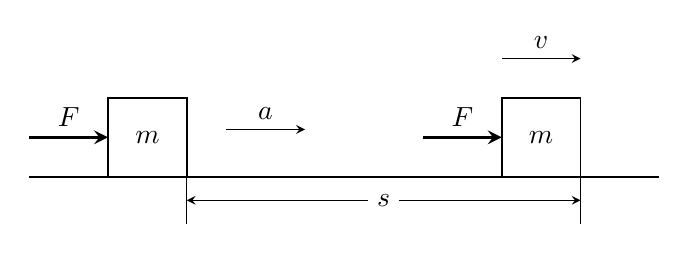
\begin{tikzpicture}[>=stealth,scale=1]
  \draw [thick] (0,0)--(8,0);
  \draw [semithick ](1,0) rectangle (2,1);  
  \draw [semithick ](6,0) rectangle (7,1);
  \node at (1.5,.5){$m$}; \node at (6.5,.5){$m$};
  \draw[->, very thick](0,.5)--node [above]{$F$}(1,.5);  
  \draw[->, very thick](5,.5)--node [above]{$F$}(6,.5);
  \draw[->](2.5,.6)--node [above]{$a$}(3.5,.6);
  \draw[->](6,1.5)--node [above]{$v$}(7,1.5);
  \draw[thin] (2,0)--(2,-.6);
  \draw[thin] (7,0)--(7,-.6);
  \draw[<->, thin](2,-.3)--node [fill=white]{$s$}(7,-.3);
\end{tikzpicture}
\end{document}